\chapter{Umsetzung}
Im Rahmen dieser Arbeit entstand eine in C++ geschriebenes Applikation welche den Marching Cubes Algorithmus auf eine Voxelmenge anwendet und das Resultat via OpgenGL visualisiert. Des Weiteren ist es möglich, das verarbeitete Model als STereoLithography (.stl) Datei zu exportieren.
\section{Marching Cubes}
\label{sec:mcUms}
Der Marching Cubes Algorithmus ist das Herzstück der entstandenen Applikation er ermöglicht die Umrechnung der gegebenen Voxel Datenmenge in eine polygonale Darstellung, welche sich im späteren Verlauf vergleichsweise einfach darstellen lässt.
\subsection{Allgemein}
Die Implementierung ist eine angepasst Version der von \citep{BourkeMC} bereitgestellten Umsetzung. Die wesentlichen Änderungen sind die Auslagerung der Funktionen in eine eigenen Klasse und das verwenden anderer Datenstrukturen. Durch die Umstellung auf STL-Behälter und der daraus folgende Verzicht auf C-Strukturen welche zur Laufzeit immer neuen Speicher anfordern, konnte die Geschwindigkeit immens gesteigert werde.
\subsection{Schnittstelle (Klasse)}
\begin{figure}[H]
	\centering
	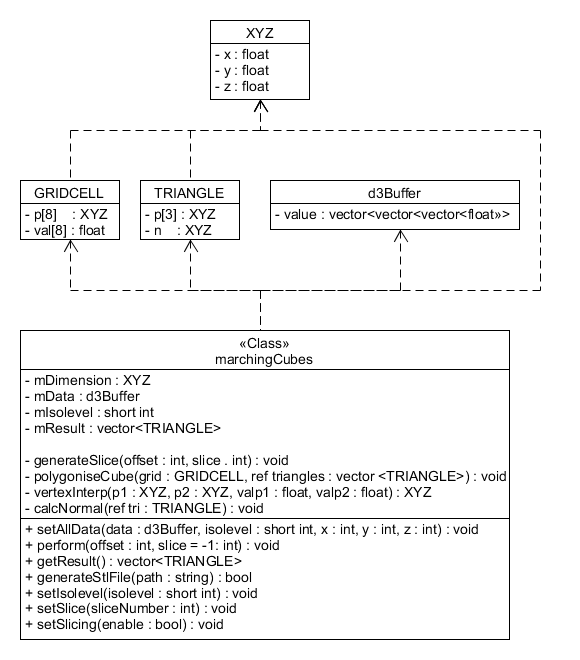
\includegraphics[width=.90\textwidth]{marchingCubes}
	\caption{UML-Diagramm der marchingCubes Klasse}
	\label{fig:marchingCubes}
\end{figure}

\subsubsection{Datentypen}
Neben den üblichen Datentypen wurden, zur leichteren Verarbeitung, komplexere Strukturen verwendet.\\
\begin{itemize}
	\item \textbf{XYZ} beschreibt einen Punkt im dreidimensionalen Raum.
	\item \textbf{GRIDCELL} ist die Repräsentation eines Voxel-Würfels. 
	\item \textbf{TRIANGLE} repräsentiert ein Dreieck mithilfe seiner drei Eckpunkte im Raum und seiner Normalen.
	\item \textbf{3dBuffer} bildet ein Voxelgitter als dreidimensionalen Vektor im Speicher ab.
\end{itemize}

\subsubsection{Funktionen}
Um ein grundlegendes Verständnis zu bieten werden hier die öffentlichen Methoden der Klasse kurz beschrieben. 
\begin{itemize}
	\item \textbf{setAllData:} Da während der Laufzeit des Programmes nur eine Instanz der marchingCubes-Klasse instanziiert wird, ist es notwendig diese, wenn nötig, mit neuen Werten zu initialisieren. Es wird das gesamte Voxelgitter (data) sowie der zu verwendende Schwellwert (isolevel) für die Berechnung mitgegeben.
	\item \textbf{perform:} Diese Funktion führt den Marching Cubes Algorithmus auf dem zuvor via setAllData gesetzten Voxelgitter aus. Es bestehen zwei Möglichkeiten des Aufrufs. Zum Einen mit beiden Parameter und zum Anderen mit nur dem ersten (offset) Parameter. Bei der ersten Variante wird nur eine Scheibe des Voxelgitters betrachtet, wobei der erste Parameter die Dicke der Scheibe und der zweite die Position der Scheibe im Gitter kennzeichnet. Bei der zweiten Variante wird der gesamte Input betrachtet wobei Parameter ''offset'' die Schrittweite pro Würfel angibt. 
	\item \textbf{getResult:} Hier kann nach dem durchlaufen von perform das Ergebnis des Algorithmus abgegriffen werden. 
	\item \textbf{setIsolevel:} Hier kann der Schwellwert der Voxeln für den Algorithmus nachträglich verändert werden.
	\item \textbf{generateStl:} Das ausführen dieser Funktion persistiert das Ergebnis des Marching Cubes Algorithmus als .stl Datei.
\end{itemize}
\subsubsection{Verwendung}
Im Programm \ref{prog:MCVerw} ist die Verwendung der Klasse exemplarisch dargestellt.
\begin{program}[H]
	\caption{Verwendung der marchingCubes Klasse}
	\label{prog:MCVerw}
	\begin{CCode}
		int main(){
			marchingCubes *mc = new marchingCubes();
			// set the voxelgrid and the treshold
			mc->setAllData(getRawData(), getIsolevel()); 
			// performs the marching cubes algorithmus on the entire voxelgrid
			mc->perform(getOffset()); 		
			// performs the algorithmus on just a slice of the voxelgrid 
			mc->perform(getOffset(), getSlice()); 
			showPolygons(mc->getResult()); 
			delete(mc);
			return 0;	
		}
	\end{CCode}
\end{program}
\section{File Formate}
Wie bereits im Kapitel \ref{sec:DateiEinf} erwähnt wurden für die Umsetzung die Dateiformate von Analyze 7.5 (.img und .hdr) sowie das STereoLithography (.stl) Format verwendet.
\subsection{Allgemein}
Um eine unnötige Komplexität zu vermeiden wurden für die Analyze-Formate nur lesender und für das STereoLithography Format nur schreibende Zugriff implementiert. Hier bieten sich für spätere Erweiterungen viele Möglichkeiten bezüglich Import/Export (auch für weitere Formate). 
\subsection{Image File (.img)}
Um das Image File auszulesen müssen vorher die Dimensionen des Voxelgitters bekannt sein.  Diese Information erhält man aus dem Header File. Sind die Dimensionen bekannt können mithilfe einer dreifach geschachtelten for-Schleife die einzelnen Voxel-Werte in eine entsprechende Datenstruktur (z.B. dreidimensionales Array) ausgelesen werden. In \citep{AnalyzeFormat} ist eine beispielhafte Implementierung gegeben. Diese wurde für den Prototyp angepasst und integriert.
\subsection{Header File (.hdr)}
Diese Datei ist wie bereits in Kapitel \ref{sec:DateiHead} beschrieben aufgebaut. Auch hier ist in \citep{AnalyzeFormat} eine beispielhafte Implementierung gegeben welche für die Verwendung angepasst und erweitert wurde.
\subsection{STereoLithography (.stl)}
In Abbildung \ref{fig:BINARYSTL} ist bereits der binäre Aufbau einer STL-Datei abgebildet. Die Implementierung (Programm \ref{prog:generateSTL}) richtet sich daher genau an diesen formalen Aufbau.
\begin{program}[H]
	\caption{Generierung einer STL-Datei}
	\label{prog:generateSTL}
	\begin{CCode}
		bool fileHandler::CreateStl(std::string path){
			FILE *fptr = NULL;
	
			int sizeResult = mResult.size();
			fprintf(stderr, "Writing triangles ...\n");
			if ((fptr = fopen(path.c_str(), "a+b")) == NULL) {
				fprintf(stderr, "Failed to open output file\n");
				return false;
			}
			char fileHeader[81] = "solid Test Head";
			char bytes[3] = { 0x00, 0x00 };
			fwrite(&fileHeader, sizeof(fileHeader)-1, 1, fptr);
			fwrite(&sizeResult, sizeof(int), 1, fptr);
			for (int i = 0; i < mResult.size(); i++) {
				fwrite(&mResult[i].n, sizeof(float), 3, fptr);
				for (int k = 0; k < 3; k++)  {
					fwrite(&mResult[i].p[k], sizeof(float), 3, fptr);
				}
				fwrite(bytes, 2, 1, fptr);
			}
			fclose(fptr);
			return true;
		}
	\end{CCode}
\end{program}
\subsection{Schnittstelle (Klasse)}
\begin{figure}[H]
	\centering
	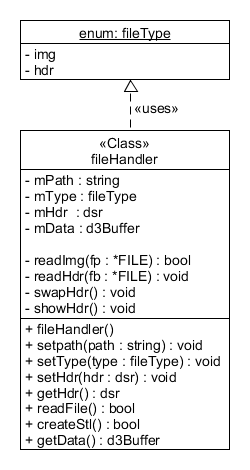
\includegraphics[width=.60\textwidth]{fileHandler}
	\caption{UML-Diagramm der fileHandler Klasse}
	\label{fig:fileHandler}
\end{figure}
\subsubsection{Datentypen}
\begin{itemize}
	\item \textbf{fileType} repräsentiert den zu verarbeitenden Dateityp als Enumeration (img bzw. hdr) 
	\item \textbf{dsr} ist die in Kapitel \ref{sec:DateiHead} beschriebene Repräsentation des Header-Formates als C-Struktur.
	\item \textbf{d3Buffer} wurde bereits im vorhergegangenen Abschnitt (\ref{sec:mcUms}) beschrieben.
\end{itemize}
\subsubsection{Funktionen}
Es folgt ein Überblick der öffentlichen Methoden dieser Klasse.
\begin{itemize}
	\item \textbf{fileHandler} der Konstruktor der Klasse initialisiert die Datenkomponenten für die spätere Verwendung.
	\item \textbf{setPath} setzt den Pfad zur verwendeten Datei.
	\item \textbf{setType} spezifiziert welche Dateityp von der Instanz dieser Klasse verwaltet werden soll.
	\item \textbf{setHdr:} Handelt es sich um eine Image-Datei sind dieser die Informationen aus der dazugehörigen Header-Datei mitzuteilen. 
	\item \textbf{getHdr:} Hier können nach dem Auslesen eines Header-File die erhaltenen Informationen abgegriffen werden. 
	\item \textbf{readFile:} Nach dem setzen von des Pfades und des Dateityps kann hier die entsprechende Datei ausgelesen werden.
	\item \textbf{createStl:} Ermöglicht das Erstellen einer .stl Datei aus den vom Marching Cubes Algorithmus gewonnen Dreiecken. 
	\item \textbf{getData:} Nach dem Auslesen einer Image-Datei können hier die erhaltenen Daten abgegriffen werden.
\end{itemize}
\subsubsection{Verwendung}
In Programm \ref{prog:fileClass} ist die beispielhafte Verwendung der fileHandler-Klasse skizziert.
\begin{program}[H]
	\caption{Verwendung der fileHandler-Klasse}
	\label{prog:fileClass}
	\begin{CCode}
		int main(){
			fileHandler *hdrFile = new fileHandler();
			fileHandler *imgFile = new fileHandler();
			
			// set the filetype
			hdrFile->setType(hdr);
			imgFile->setType(img);
			
			// set the file path
			hdrFile->setPath(ui->headerPath->text().toStdString());
			imgFile->setPath(ui->imagePath->text().toStdString());
			
			// read the header file
			hdrFile->readFile();
			// set the header for the image file
			imgFile->setHdr(hdrFile->getHdr());
			// read the image file
			imgFile->readFile();
			
			// get the image data and pass it to the marching cubes algorithm
			marchingCubes->setData(imgFile->getData());
			
			delete(hdrFile);
			delete(imgFile);
			return 0;	
		}
	\end{CCode}
\end{program}
\section{OpenGL}
Für die grafische Aufbereitung des generierten polygonalen Objektes wird wie bereits mehrfach erwähnt OpenGL verwendet. Um eine möglichst große Unabhängigkeit bezüglich des gewählten Betriebssystemes zu gewährleisten wurde QT als Schnittstelle zwischen System und OpenGL gewählt.
\subsection{Allgmein}
Die Implementierung ermöglicht die Darstellung des generierten Objektes, das bewegen um die Achsen via Maus sowie das Zoomen via Mausrat.
\subsection{Schnittstelle (Klasse)}
\begin{figure}[H]
	\centering
	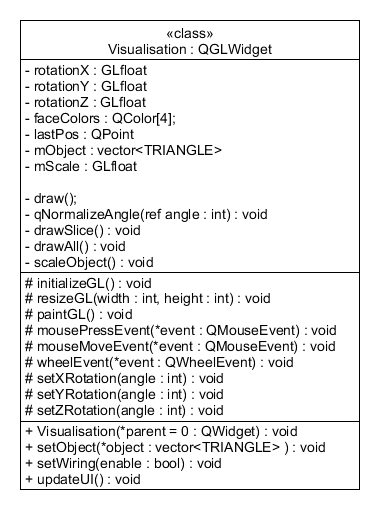
\includegraphics[width=.70\textwidth]{visualisation}
	\caption{UML-Diagramm der Visualisation Klasse}
	\label{fig:visualisation}
\end{figure}
\subsubsection{Funktionen}
\begin{itemize}
	\item \textbf{Visualisation:} Erstellen der Zeichenoberfläche.
	\item \textbf{setObject:} Setzen des zu zeichnenden Objektes.
	\item \textbf{setWiring:} Ermöglicht das hin -und herschalten zwischen den beiden Polygonmodi GL\_LINE und GL\_FILL (s. Abbildung \ref{fig:UIWiring}).
	\item \textbf{updateUI:} Manuelles update der Zeichenfläche z.B. nach setWiring oder setObjekt um die Änderungen für den Benutzer sichtbar zu machen.
\end{itemize}
\subsubsection{Verwendung}
Die Verwendung dieser Klasse ist vergleichsweise einfach. Eine beispielhafte Implementierung ist in Programm \ref{prog:VisVerw} zu finden.
\begin{program}[H]
	\caption{Exemplarische Verwendung der Visualisation Klasse}
	\label{prog:VisVerw}
	\begin{CCode}
		int main(){
			Visualisation vi = new Visualisation();
			// set the polygon object (result of the marching cubes algorithm)
			vi->setObject(marchingCubes->getResult());
			// update ui for the user
			vi->updateUI;
			// enable wiring (set polygon mode to GL\_LINE)
			vi->setWiring(true);
			// update ui for the user
			vi->updateUI;
			delete(vi);
		} 
	\end{CCode}
\end{program}

\section{Benutzeroberfläche}
In diesem Abschnitt wird auf die Funktionen der Benutzeroberfläche (UI) des entstandenen Prototypen eingegangen. Erstellt wurde diese mithilfe des QT-Designers. Um eine einfache Benutzung zu gewährleisten wurde sie möglichst schlicht gehalten.

\subsection{Allgemeiner Aufbau}
In Abbildung \ref{fig:UI1} ist die Benutzeroberfläche dargestellt. Es folgt nun eine kurze Beschreibung der einzelnen Schaltflächen.
\begin{itemize}
	\item \textbf{Menu:} In der linken oberen Ecke befindet sich die Menu Schaltfläche welche nur einen Eintrag aufweist. Dieser ermöglicht das Exportieren des generierten Objektes in das .stl Format.
	\item \textbf{Select Header:} Durch das betätigen des Button ''Select Header'' öffnet sich eine Dialogbox zum Auswählen einer .hdr Datei im Dateisystem. Nach erfolgreichem selektieren einer Datei erscheint der Dateipfad links im Textfeld. Alternativ kann auch der Pfad direkt im Textfeld bearbeitet werden.
	\item \textbf{Select Image:} Die Funktionalität ist Analog zu ''Select Header'' für .img Dateien.
	\item \textbf{Generate View:} Durch das betätigen dieser Schaltfläche wird der Marching Cubes Algorithmus auf die ausgewählten Dateien angewandt. Nach erfolgreicher Berechnung wird das Ergebnis rechts in der Zeichenoberfläche dargestellt.
	\item \textbf{Enable Wiring:} Siehe Abschnitt \ref{sec:slicing}.
	\item \textbf{Enable Slicing:} Siehe Abschnitt \ref{sec:wiring}.
	\item \textbf{Zeichenoberfläche:} Die rechte Hälfte der Benutzeroberfläche dient zur dreidimensionalen Darstellung des generierten Objektes. Mithilfe der Maus ist es möglich das angezeigte Objekt zu rotieren. Des Weiteren besteht die Möglichkeit mit dem Mausrat die Größe zu ändern (zoomen).
	\item \textbf{Isolevel Regler:} Der rechts neben der Zeichenfläche angebrachte Regler dient zur Anpassung des Isowertes. Bei jeder Änderung wird das anzuzeigende Objekt mit dem neuen Wert berechnet und angezeigt.
	\item \textbf{Polygon Regler:} Dieser Regler ist unterhalb der Zeichenoberfläche zu finden und hat zwei Funktionen. Die erste Funktionalität ist das anpassen der Schrittweite für den Marching Cubes Algorithmus. Eine höhere Schrittweite führt zu einer gröberen polygonalen Struktur. Die zweite Funktion ist das anpassen der Dicke der Scheibe bei aktiviertem ''Slicing''
\end{itemize}
\begin{figure}[H]
	\centering
	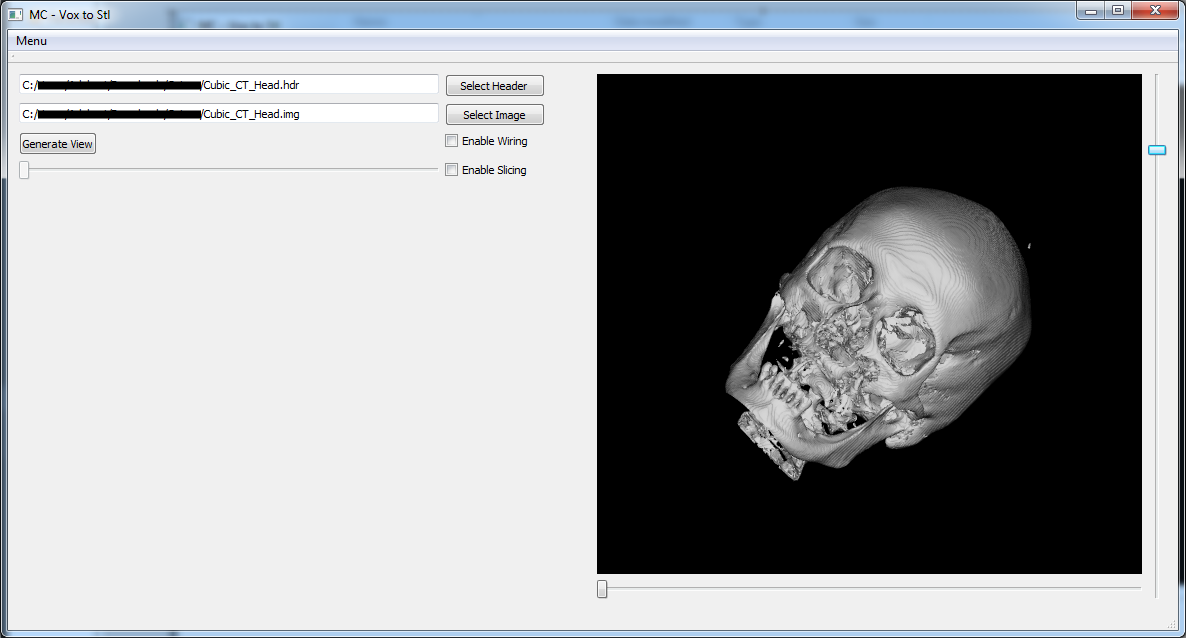
\includegraphics[width=1.0\textwidth]{UI1}
	\caption{Übersicht der Benutzeroberfläche}
	\label{fig:UI1}
\end{figure}
\subsection{Slicing}
\label{sec:slicing}
Die Schaltfläche ''Enable Slicing'' ermöglicht die Darstellung einer einzelnen Scheibe des gesamt Objektes. Durch das Aktivieren der Checkbox wird auch der Regler links Aktiviert. Mithilfe von diesem kann das zu betrachtende Scheibenelement verschoben werden. Des Weiteren ändert sich die Funktionalität des unteren Reglers von der Regulierung der Polygongröße zur Regulierung der Dicke der Scheibe.\\
\\
Vorteil dieser Darstellungsform ist das mit aktivem Slicing das Innenleben eines Objektes betrachtet werden kann.\\
\\
Das Benutzerinterface mit Aktiviertem Slicing ist in Abbildung \ref{fig:UISlicing} zu sehen.
\begin{figure}[H]
	\centering
	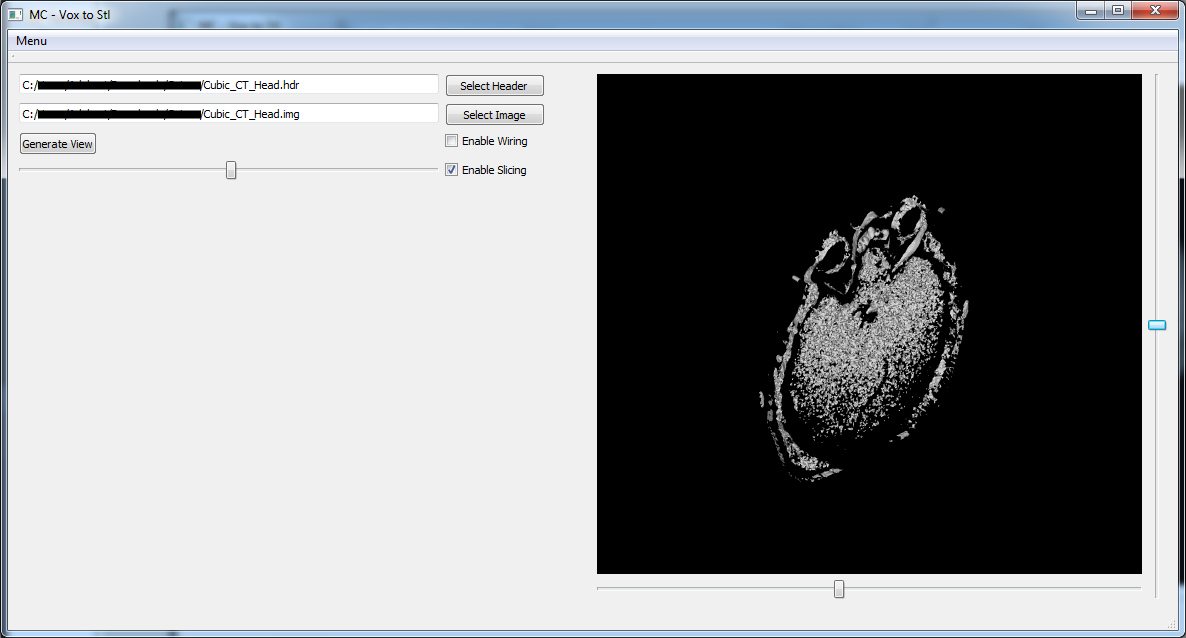
\includegraphics[width=1.0\textwidth]{UISlicing}
	\caption{Programm Slicing aktiviert}
	\label{fig:UISlicing}
\end{figure}
\subsection{Wiring}
\label{sec:wiring}
Durch Aktivieren der Checkbox ''Enable Wiring'' kann das Drahtgittermodell des Objektes betrachtet werden. Diese Darstellung ermöglicht es die polygonale Struktur des Objektes besser zu erkennen. In Abbildung \ref{fig:UIWiring} ist ein Objekt mit aktiven Wiring zu sehen.
\begin{figure}[H]
	\centering
	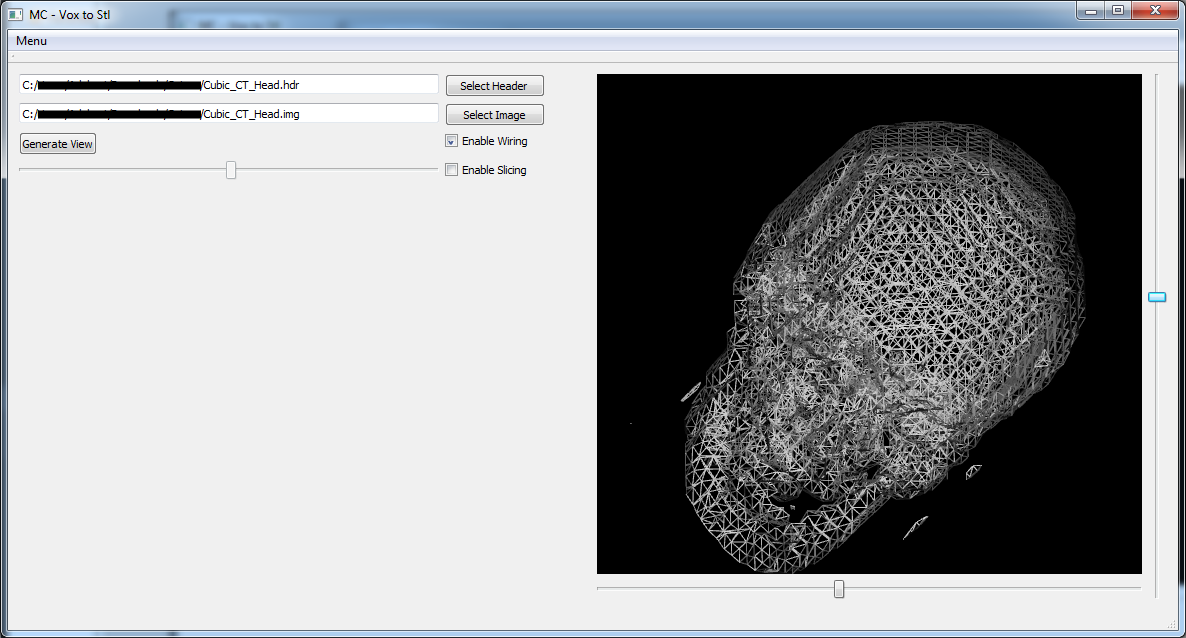
\includegraphics[width=1.0\textwidth]{UIWiring}
	\caption{Programm Wiring aktiviert}
	\label{fig:UIWiring}
\end{figure}